% RENDER this using Overleaf due to {fancyhdr}
\documentclass{article}
\usepackage{fancyhdr}
% Set up the custom footer
\pagestyle{fancy}
\fancyfoot[R]{\thepage} % Centered page number in footer
\fancyfoot[C]{\textbf{License:} CC-BY.\textbf{Copyright:} Andree \& Degoot, 2025 }
\usepackage{booktabs} % to render table
\usepackage{tikz}
\usetikzlibrary{arrows.meta, positioning}
\usepackage{amsmath}
\author{Andree Valle Campos and Abdoelnaser M Degoot \\ Epiverse-TRACE Team @ LSHTM }
\title{Simple Introduction to Mathematical Modelling of Infectious Diseases}
\begin{document}
\maketitle

\section{Introduction}
This practical aims to assess your understanding of the fundamental
principles of mathematical modeling while guiding you in constructing models using
a simple SEIR framework for infectious disease outbreaks.\\

 \textbf{Note: Please fill in the blanks.}

\section{SEIR Model}

 In the  SEIR model, we have four compartments (\( S \), \( E \), \( I \), \( R \)):

\begin{itemize}
    \item \( S \) stands for \underline{\hspace{2cm}}, meaning \underline{\hspace{6cm}}.
The parameter that explains the transition from  (\( S \)) compartment
to  (\( E \)) compartment is \underline{\hspace{6cm}}.
\item \(E\) stands for \underline{\hspace{2cm}}, meaning that it can
    \underline{\hspace{4cm}}.

    The rate that explains the transition from  (\( E \)) to  (\( I \)) is the rate of \underline{\hspace{1cm}}.

    \item \( I \) stands for \underline{\hspace{2cm}}, meaning that it can
    \underline{\hspace{4cm}}.
    The rate that explains the transition from  (\( I \)) to  (\( R \)) is the rate of \underline{\hspace{1cm}}.

    \item \( R \) stands for \underline{\hspace{3cm}}. This compartment includes those who have ceased to be infectious and acquire immunity against infection, regardless of the clinical course.
\end{itemize}

\section{\( R_0 \)}
\( R_0 \) helps project the potential
size of an epidemic and calculate the herd immunity threshold.
It is defined as the average number of secondary \underline{\hspace{2cm}} generated from a primary case in a completely
\underline{\hspace{3cm}} population.

\section{\( R_t \)}
\( R_t \)
helps monitor the progress of the epidemic.
When the population is no longer \underline{\hspace{2cm}}, the instantaneous
reproduction number \( R_t \) is used. This is defined as the average number
of s\underline{\hspace{2cm}} in a population composed of
\underline{\hspace{2cm}} and non-\underline{\hspace{2cm}} individuals at time \( t \).

\section{A Diagram for Measles outbreak}

Below is a typical SEIR model with demography (births and deaths). This is a simple
model applicable to person-to-person infections in a homogeneously mixing population.
Please carefully observe the model and examine the interactions with the equations
in section \ref{eqs}.  Use color codes or arrows to relate the diagram to the equations.


\begin{center}
    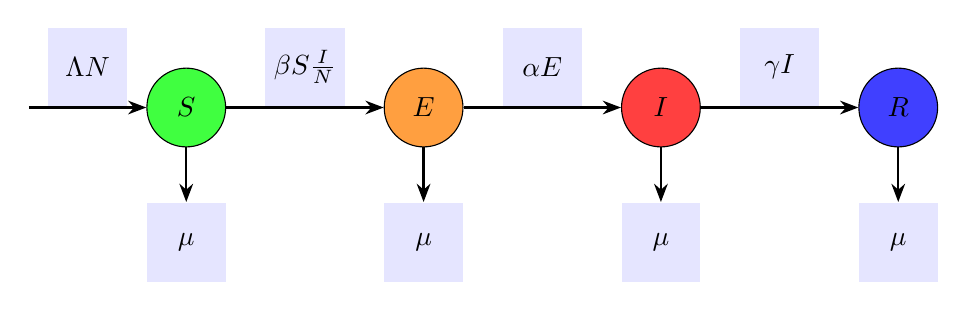
\begin{tikzpicture}[
        node distance=2cm,
        every node/.style={fill=blue!10, draw, minimum size=1cm, text centered},
        arrow/.style={-Stealth, thick}
    ]

    % Nodes
    \node [circle, fill=green!75](S) {$S$};
    \node [circle, fill=orange!75](E) [right=of S] { $E$};
    \node [circle, fill=red!75](I) [right=of E] {$I$};
    \node [circle, fill=blue!75](R) [right=of I] {$R$};

    % Arrows for transitions
    \draw[arrow] (S) -- node[above, draw=none] {$\beta S  \frac{I}{N}$} (E);
    \draw[arrow] (E) -- node[above, draw=none] {$\alpha  E$} (I);
    \draw[arrow] (I) -- node[above, draw=none] {$\gamma  I$} (R);

    % Natural birth and death rates
    \draw[arrow] (-2,0.0) -- node[above, draw=none] {$\Lambda N$} (S);
    \draw[arrow] (S) -- +(0,-1.2) node[below, draw=none] {$\mu$};
    \draw[arrow] (E) -- +(0,-1.2) node[below, draw=none] {$\mu$ };
    \draw[arrow] (I) -- +(0,-1.2) node[below, draw=none] {$\mu$ };
    \draw[arrow] (R) -- +(0,-1.2) node[below, draw=none] {$\mu$};

    \end{tikzpicture}
\end{center}

Where:
\begin{itemize}
    \item \( \beta \): Transmission rate
    \item \( \alpha \): Infectiousness rate, or rate of progression from exposed to infectious
    \item \( \gamma \): Recovery rate
    \item \( \mu \): Death rate (natural death rate)
    \item \( N \): Total population size, \( N = S + E + I + R \).
\end{itemize}

 The parameter $\beta$, defined as the average rate at which infectious individuals can infect susceptibles,
 is derived from the multiplication of $p$
 and $c$, where $p$ is the probability of transmission during contact, and $c$
 is the contact rate, defined as the average number of contacts per unit of time.\\

 If a transmission rate $\beta$ equals 3, it means
each infectious individual causes 3 new infections per day
in a fully susceptible population.\\

Model parameters are often (but not always) specified as rates.
The rate at which an event occurs is the inverse of the average time until that event.
For example, in the SEIR model, the recovery rate $\gamma$ is the inverse of the average infectious period.\\

Values of these rates can be determined from the natural history of the disease.
For example,  if people are on average infectious for 8 days, then in the model,
1/8 of currently infectious people would recover each day
(i.e. the rate of recovery, $\gamma=1/8=0.125$).

\section{Equations}\label{eqs}
Note that in the diagram, arrows entering compartments are expressed as positive
terms in the equations, while arrows exiting compartments are represented with negative terms.
Based on the above diagram,deduce the following equations that describe this system:

\section*{Compartment Equations}

\begin{itemize}
    \item \textbf{S compartment:}
    \[
    \frac{dS}{dt} =
    \]

    \item \textbf{E compartment:}
    \[
    \frac{dE}{dt} =
    \]
    \item \textbf{I compartment:}
    \[
    \frac{dI}{dt} = \
    \]

    \item \textbf{R compartment:}
    \[
    \frac{dR}{dt} =
    \]
\end{itemize}

\section{Parameters for the Measles outbreak}
A parameter within a transmission model
corresponds to a biological or social property of a dynamic system
for a specific context.
In this section we will give the elements to feed the parameters
of a SEIR model for a Measles outbreak in Burkina Faso.
\begin{itemize}
	\item The average latent period (or pre-infectious) for measles is
	around 8 days (Masters et al., 2023).
	\item The average infectious period lasts for 5 days (Masters et al., 2023).
	\item For measles the basic reproduction number typically ranges
	from 12 to 18, or even more (Fiona et al., 2017).
	\item A single infectious case is introduced into the population.
	\item The entire population, except for this one case, is initially susceptible.
	This assumption simplifies the model and allows us to explore the spread of
	infection in the absence of immunity. Although real populations typically
	have some immunity due to vaccination or prior infection.
	Also, no individuals are exposed or recovered at this moment.
	\item The population of Burkina Faso is approximately $N\approx 22.67$ million.
	\item The age structure of Burkina Faso is characteristic of a young
	population, with a majority of the population being under 25 years old.
	According to recent estimates (United Nations, 2023;
	Central Intelligence Agency, 2023); World Bank, 2023),
	the age structure is broken down as follows:

	\begin{itemize}
	\item $[0\to15)$ years: $\sim 44 \, (43-45)$\% of the population
	\item $[15\to 25)$ years: $\sim 19.5 \, (19-20)$\%
	\item $[25\to 55)$ years: $\sim 29 \, (28-30)$\%
	\item $[55\to 65)$ years: $\sim 5 \, (3-5)$\%
	\item $65+$ years : $\sim 2.5 \, (2-3)$\%
	\end{itemize}

\end{itemize}
\section{Table of parameters}
Please fill in the table below with the parameters described above.
Additionally, please note that we will do the simulation for 120 days.
% Please add the following required packages to your document preamble:
% \usepackage{booktabs}
\begin{table}[htb]
	\centering
	\addtolength{\leftskip} {-2cm}
	\addtolength{\rightskip}{-2cm}
	\begin{tabular}{@{}lll@{}}
		\toprule
		Parameter            & Value              & Definition                                                                            \\ \midrule
		bf\_pop              & \underline{\hspace{1cm}} & Population size                                                                       \\
		S/N                    & \underline{\hspace{1cm}}  & Proportion of Susceptibles                                                            \\
		E/N                    &  \underline{\hspace{1cm}} & Proportion of Exposed                                                                 \\
		I/N                    & \underline{\hspace{1cm}} & Proportion of Infectious                                                              \\
		R/N                    & \underline{\hspace{1cm}} & Proportion of Recovered                                                               \\
		V/N                    & \underline{\hspace{1cm}} & Proportion of Vaccinated                                                              \\
		r0                   & \underline{\hspace{1cm}} & Basic reproduction number                                                             \\
		latent\_period       & \underline{\hspace{1cm}} & Time between becoming infected and the onset of infectiousness (in days)             \\
		infectious\_period   & \underline{\hspace{1cm}} & Time between the onset and end of infectious viral shedding (in days)                \\
		transmission\_rate   & \underline{\hspace{1cm}}  & Rate at which infectious individuals can infect susceptibles (r0/infectious\_period) \\
		infectiousness\_rate &  \underline{\hspace{1cm}}  & Rate of progression from exposed to infectious (1/latent\_period)                    \\
		recovery\_rate       & \underline{\hspace{1cm}}  & Rate of progression from infectious to recovered (1/infectious\_period)              \\
		time\_end            & \underline{\hspace{1cm}} & Maximum number of timesteps over which to run the model (in days)                     \\
		increment            & \underline{\hspace{1cm}}  & The size of the time increment (in days)                                              \\ \bottomrule
	\end{tabular}
\end{table}

\section{Computing $R_0$}
The expression for the basic reproduction number ($R_0$) in the above system  is given by:

\begin{equation*} R_0 = \frac{\mu}{(\mu + \alpha)} \frac{\beta}{(\mu + \gamma)}. \end{equation*}

To calculate the $R_0$ value for given parameter values,  write an R object
called Measles$R_0$ that implements this formula. The function will use the following parameter values:

    \begin{itemize}
        \item $\mu = \frac{1}{75}$ (natural mortality rate)
        \item $\alpha = \frac{1}{10}$ (rate of progression from the exposed to the infectious stage)
        \item $\gamma = 1/8$ (recovery rate)
        \item $\beta = 1.8$ (transmission rate)
    \end{itemize}
Then compute the final size of such epidemic.

\section{About this document}
We adapted this material from "Practical: building a simple compartmental model for Zika" by Zulma Cucunubá, Pierre Nouvellet, and José M. Velasco-España, 2024-01-10 (V.1.0.3.).
License: CC-BY 4.0 by the authors.
For more details, visit: https://epiverse-trace.github.io/tutorials-late/LICENSE.html


\end{document}
